\documentclass[11pt,a4paper]{article}
\usepackage[left=3cm,right=2.5cm,top=2.6cm,bottom=2.6cm]{geometry}
\usepackage[T1]{fontenc}
\usepackage[utf8]{inputenc}
\usepackage{lmodern}
\usepackage{amsmath,amssymb}
\usepackage{graphicx,float}
\usepackage{booktabs,tabularx,array}
\usepackage{xcolor,listings}
\usepackage{setspace,enumitem}
\usepackage{fancyhdr}
\usepackage{caption}
\usepackage{hyperref}
\usepackage{microtype}

\definecolor{navy}{HTML}{18364F}
\definecolor{muted}{HTML}{52616F}
\definecolor{codebg}{HTML}{F4F6F8}
\definecolor{linegray}{HTML}{D5DDE4}
\hypersetup{
  colorlinks=true,linkcolor=navy,urlcolor=navy,citecolor=navy,
  pdftitle={Laporan UTS INF301 - Kelompok 9 - Nomor 1 dan 3},
  pdfauthor={Bambang Herlambang; Dustin Pranata Wangsawidjaja}
}
\urlstyle{same}
\setstretch{1.1}
\setlength{\parindent}{1.2em}
\setlength{\parskip}{3pt}
\setlength{\headheight}{14pt}
\emergencystretch=2em
\setlist{itemsep=2pt,topsep=4pt,leftmargin=*}
\captionsetup{font=small,labelfont=bf,labelsep=period}
\renewcommand{\contentsname}{Daftar Isi}
\renewcommand{\figurename}{Gambar}
\renewcommand{\tablename}{Tabel}
\renewcommand{\refname}{Daftar Pustaka}
\renewcommand{\lstlistingname}{Kode}
\DeclareRobustCommand{\kode}[1]{{\urlstyle{tt}\nolinkurl{#1}}}

\lstdefinestyle{pythoncode}{
  language=Python,basicstyle=\ttfamily\footnotesize,
  keywordstyle=\color{navy}\bfseries,commentstyle=\color{muted},
  stringstyle=\color{teal!60!black},numbers=left,
  numberstyle=\tiny\color{muted},numbersep=8pt,
  breaklines=true,breakatwhitespace=false,columns=fullflexible,
  keepspaces=true,showstringspaces=false,tabsize=4,
  frame=single,rulecolor=\color{linegray},backgroundcolor=\color{codebg},
  framesep=6pt,aboveskip=10pt,belowskip=10pt
}
\lstdefinestyle{pseudocode}{
  style=pythoncode,language={},numbers=none,basicstyle=\ttfamily\small
}
\lstdefinestyle{terminal}{
  style=pythoncode,language={},numbers=none,basicstyle=\ttfamily\footnotesize
}
\pagestyle{fancy}
\fancyhf{}
\fancyhead[L]{\small INF301 -- Pengolahan Citra Digital}
\fancyhead[R]{\small Kelompok 9}
\fancyfoot[C]{\small \thepage}
\renewcommand{\headrulewidth}{0.4pt}
\raggedbottom

\begin{document}
\hypersetup{pageanchor=false}
\newgeometry{left=3cm,right=3cm,top=3cm,bottom=3cm}
\begin{titlepage}
\begingroup
\centering
\fontfamily{ptm}\selectfont
\fontsize{14}{16}\selectfont
\setstretch{1}
\setlength{\parskip}{0pt}
{\bfseries LAPORAN UJIAN TENGAH SEMESTER\par}
\vspace{1cm}
{\bfseries PENGOLAHAN CITRA DIGITAL (INF301)\par}
\vspace{0.15cm}
{\bfseries PENYELESAIAN SOAL NOMOR 1 DAN 3\par}
\vspace{0.4cm}

\includegraphics[width=10cm]{images/logo-ukwms.png}\par
\vspace{0.7cm}
{\bfseries ANGGOTA TIM\par}
\vspace{0.35cm}
{\fontsize{12}{14}\selectfont
\begin{tabular}{@{}l@{\hspace{1.3cm}}l@{}}
Bambang Herlambang & 5803024019\\
Dustin Pranata Wangsawidjaja & 5803024021\\
\end{tabular}
\par}
\vfill
{\bfseries
PROGRAM STUDI INFORMATIKA\par
\vspace{0.3cm}
FAKULTAS TEKNIK\par
\vspace{0.3cm}
UNIVERSITAS KATOLIK WIDYA MANDALA\par
\vspace{0.3cm}
SURABAYA\par
\vspace{0.3cm}
2026\par}
\endgroup
\end{titlepage}
\restoregeometry

\pagenumbering{roman}
\hypersetup{pageanchor=true}
\tableofcontents
\clearpage
\pagenumbering{arabic}

\section{Pendahuluan}

\subsection{Latar belakang dan tujuan}
Pengolahan citra digital memungkinkan perubahan intensitas, pemisahan objek,
dan pengukuran bentuk dilakukan secara komputasional. Laporan ini membahas
penyelesaian tiga bagian Ujian Tengah Semester mata kuliah Pengolahan Citra
Digital, yaitu selisih respons \textit{Laplacian of Gaussian} pada soal nomor 1,
segmentasi karakter pada soal nomor 2, serta penghitungan koin menurut ukuran pada soal nomor 3 \cite{soal-uts}.

Tujuan pekerjaan adalah mengimplementasikan algoritma dalam Python,
menjelaskan tahapan dan dasar matematisnya, serta memeriksa hasil dengan data
contoh dan pengujian otomatis. Pembahasan nomor 1 mempertahankan standar
deviasi yang tertulis pada soal, yaitu $0{,}1$ dan $0{,}2$. Pembahasan nomor 3
menggunakan fungsi \kode{regionprops} untuk mengukur setiap objek koin yang
telah dipisahkan.

\subsection{Ruang lingkup dan data}
Laporan ini mencakup nomor 1, 2, dan 3. Kode, citra masukan, serta hasil
perhitungan tersimpan dalam direktori masing-masing soal. Nomor 1 dan 3 dikerjakan oleh Bambang Herlambang (5803024019),
sedangkan nomor 2 dikerjakan oleh Dustin Pranata Wangsawidjaja (5803024021).

\begin{table}[H]
\centering
\caption{Bahan masukan dan implementasi yang digunakan.}
\label{tab:bahan}
\small
\begin{tabularx}{\textwidth}{@{}p{2.1cm}X@{}}
\toprule
\textbf{Bagian} & \textbf{Bahan dan program}\\
\midrule
Nomor 1 &
Citra sintetis grayscale $384 \times 256$ piksel pada
\path{soal1/data/citra_uji.png}; program \path{soal1/main.py}.\\
\addlinespace
Nomor 2 & Citra teks pada \path{soal2/teks.png}; program
\path{soal2/main.py}, dikerjakan oleh Dustin.\\
\addlinespace
Nomor 3 &
Citra sintetis $1100 \times 1100$ piksel berisi 100 koin terpisah pada
\path{soal3/data/koin_100.png}; program \path{soal3/main.py}.\\
\addlinespace
Validasi &
Metadata koin pada \path{soal3/data/koin_100_ground_truth.json} serta
pengujian pada \path{soal1/tests/} dan \path{soal3/tests/}.\\
\bottomrule
\end{tabularx}
\end{table}

Citra contoh nomor 1 dan 3 dibuat secara sintetis melalui \path{buat_data_contoh.py}
dengan \textit{seed} 9 agar dapat direproduksi. Citra koin bukan foto uang
logam nyata. Data acuan atau \textit{ground truth} hanya dipakai untuk
memeriksa hasil; program penghitung membaca citra tanpa mengambil jumlah
atau ukuran koin dari metadata acuan.

Kode lengkap dan berkas pendukung tersedia pada
\href{https://github.com/Bambang-code/uts-pcd-kelompok-9}{repositori GitHub Kelompok 9}.
Langkah pemasangan dan pelaksanaan disajikan pada
Bagian~\ref{sec:reproduksi}.

\clearpage
\section{Penyelesaian Soal Nomor 1: Selisih LoG}
\label{sec:soal1}

\subsection{Tujuan dan asumsi}

Soal nomor 1 meminta pembacaan citra, penerapan filter Laplacian Gaussian
dengan standar deviasi $0{,}1$ dan $0{,}2$, serta penyimpanan kedua respons
dan selisihnya \cite{soal-uts}. Istilah LG diinterpretasikan sebagai
\textit{Laplacian of Gaussian} (LoG). Standar deviasi dinyatakan dalam
\textbf{piksel} pada kedua sumbu, sedangkan selisih didefinisikan sebagai
\texttt{im1 - im2}. Nilai parameter tersebut dipertahankan sesuai soal.

Masukan RGB diubah menjadi grayscale agar filter bekerja pada dua dimensi
spasial. Transparansi RGBA dikompositkan ke putih sebelum konversi warna.
Intensitas citra dinyatakan sebagai \kode{float64} dalam rentang $[0,1]$.
Program menolak masukan kosong, dimensi yang tidak didukung, dan intensitas
yang tidak berhingga. Data contoh berukuran $384 \times 256$ piksel dan
tersedia pada \kode{soal1/data/citra_uji.png}.

\subsection{Dasar matematis}

Gaussian dua dimensi dengan standar deviasi $\sigma$ dinyatakan sebagai
\begin{equation}
G_\sigma(x,y)=\frac{1}{2\pi\sigma^2}
\exp\!\left(-\frac{x^2+y^2}{2\sigma^2}\right).
\end{equation}
Untuk citra intensitas $I$, respons LoG kontinu adalah
\begin{equation}
L_\sigma=\nabla^2(G_\sigma * I)
=\frac{\partial^2(G_\sigma * I)}{\partial x^2}
+\frac{\partial^2(G_\sigma * I)}{\partial y^2},
\end{equation}
dengan $*$ menyatakan konvolusi. Implementasi diskret menggunakan
\kode{scipy.ndimage.gaussian_laplace}, yaitu penjumlahan turunan kedua
Gaussian pada setiap sumbu \cite{scipy-log}. Perluasan batas memakai
\kode{reflect}. Tidak diterapkan perkalian tambahan dengan $\sigma^2$
karena normalisasi skala tersebut tidak diminta dalam soal. Keluaran
yang dihitung adalah
\begin{equation}
\mathrm{im1}=L_{0.1},\qquad
\mathrm{im2}=L_{0.2},\qquad
D=\mathrm{im1}-\mathrm{im2}.
\end{equation}

\clearpage
\subsection{Algoritma dan implementasi}

Program mengikuti empat langkah pada soal sebagai berikut.
\begin{enumerate}[label=\alph*.,leftmargin=*,itemsep=2pt]
\item \textbf{Baca citra (image).} Citra dibaca dari berkas masukan,
diubah menjadi grayscale bila diperlukan, lalu dinormalisasi sebagai
\kode{float64} dalam rentang $[0,1]$.
\item \textbf{Gunakan filter LoG dengan standar deviasi $0{,}1$.}
Terapkan filter pada citra masukan yang telah disiapkan, lalu simpan
respons sebagai \kode{im1}.
\item \textbf{Gunakan filter LoG dengan standar deviasi $0{,}2$.}
Terapkan filter pada citra masukan yang sama, bukan pada \kode{im1},
lalu simpan respons sebagai \kode{im2}.
\item \textbf{Tentukan selisih dan simpan sebagai citra hasil.}
Program menghitung \kode{hasil = im1 - im2} pada array \kode{float64}
bertanda sebelum pemetaan tampilan. Keluaran disimpan sebagai
\kode{hasil.npy} dan pratinjau citra \kode{hasil.png}.
\end{enumerate}

Langkah a--d dirangkum dalam kode semu berikut.

\noindent\begin{minipage}{\textwidth}
\begin{lstlisting}[style=pseudocode,caption={Kode semu penyelesaian nomor 1.}]
MULAI
    BACA citra
    JIKA RGBA: kompositkan ke latar putih
    JIKA RGB: ubah menjadi grayscale
    KONVERSI intensitas ke float64 dalam [0, 1]
    im1 <- FILTER_LOG(citra, sigma=0.1, batas=reflect)
    im2 <- FILTER_LOG(citra, sigma=0.2, batas=reflect)
    hasil <- im1 - im2
    SIMPAN im1, im2, hasil sebagai array float64
    HITUNG batas tampilan bersama dari ketiga respons
    SIMPAN PNG pratinjau dan metadata parameter
SELESAI
\end{lstlisting}
\end{minipage}

Berikut inti fungsi \kode{hitung_selisih_log} pada \kode{soal1/main.py}.
Nilai bawaan \kode{sigma_1} dan \kode{sigma_2} adalah $0{,}1$ dan $0{,}2$;
pengurangan dilakukan sebelum penyesuaian tampilan.

\noindent\begin{minipage}{\textwidth}
\begin{lstlisting}[style=pythoncode,caption={Perhitungan kedua respons dan selisihnya.}]
im1 = gaussian_laplace(citra, sigma=sigma_1, mode="reflect")
im2 = gaussian_laplace(citra, sigma=sigma_2, mode="reflect")
hasil = im1 - im2
return im1, im2, hasil
\end{lstlisting}
\end{minipage}

\subsection{Penyimpanan dan hasil pengolahan}

Keluaran utama \kode{im1.npy}, \kode{im2.npy}, dan \kode{hasil.npy}
menyimpan array \kode{float64} bertanda. Konversi langsung ke
\kode{uint8} sebelum pengurangan dapat menghilangkan informasi negatif.
File PNG digunakan untuk pratinjau, sedangkan file \kode{.npy} menjadi
acuan perhitungan lanjutan. Semua keluaran bawaan disimpan di
\kode{soal1/hasil/}.

Ketiga PNG respons menggunakan rentang bersama $[-M,M]$, dengan $M$
merupakan nilai absolut terbesar dari seluruh piksel ketiga array.
Jika ketiganya nol, digunakan $M=1$. Pemetaan tampilan dinyatakan sebagai
\begin{equation}
q(F)=\operatorname{round}\!\left[
\frac{255}{2}\left(\operatorname{clip}(F/M,-1,1)+1\right)\right].
\end{equation}
Nilai nol ditampilkan sebagai abu-abu 128. Nilai negatif lebih gelap dan
nilai positif lebih terang. Pemetaan ini tidak mengubah array asli.

\begin{figure}[H]
\centering
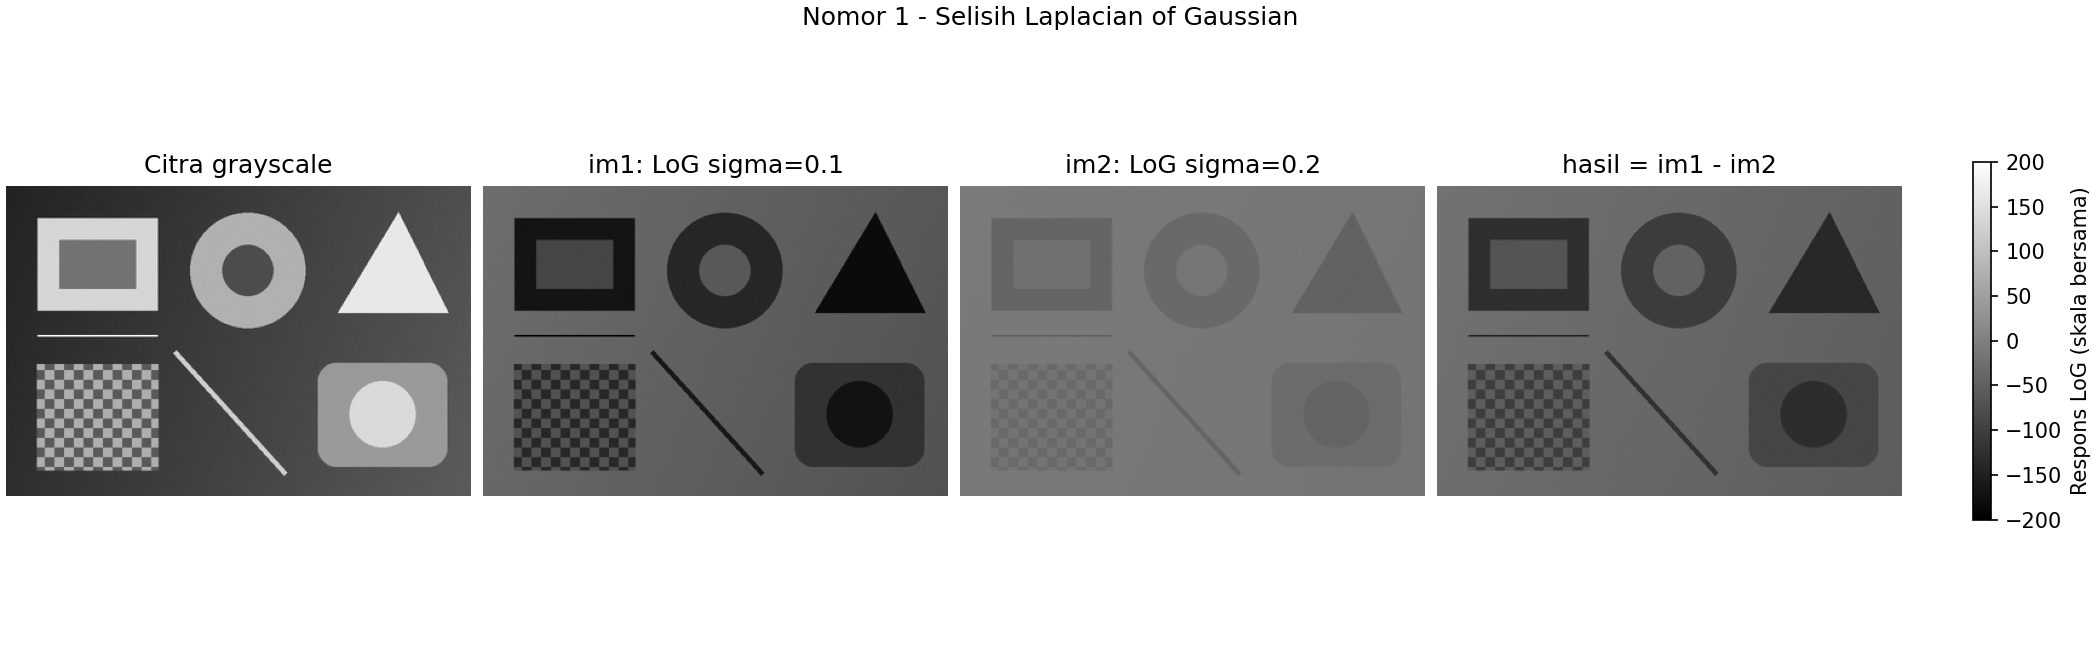
\includegraphics[width=\textwidth]{images/log-perbandingan.png}
\caption{Citra grayscale dan hasil pengolahan nomor 1. Ketiga respons
memakai skala bersama, sedangkan citra grayscale memakai rentang $[0,1]$.}
\label{fig:log-perbandingan}
\end{figure}

\begin{table}[H]
\centering
\caption{Rentang respons asli pada citra contoh, dibulatkan enam desimal.}
\label{tab:log-rentang}
\begin{tabular}{@{}lrr@{}}
\toprule
\textbf{Array} & \textbf{Minimum} & \textbf{Maksimum} \\
\midrule
\kode{im1} & $-200{,}000000$ & $-18{,}039216$ \\
\kode{im2} & $-49{,}994045$ & $-4{,}507871$ \\
\kode{hasil} & $-150{,}006577$ & $-13{,}531345$ \\
\bottomrule
\end{tabular}
\end{table}

Tabel~\ref{tab:log-rentang} berasal dari \kode{metadata.json}, yang juga
mencatat sigma, ukuran citra, metode batas, dan rentang PNG. Pada data
contoh ini $M$ sekitar 200 dan seluruh respons bernilai negatif. Karena
skala tampilan dipakai bersama, perbedaan kecerahan antarpanel pada
Gambar~\ref{fig:log-perbandingan} mencerminkan perbedaan besar respons.

\subsection{Interpretasi sigma kecil dan keterbatasan}

LoG kontinu ideal memberikan respons nol pada citra konstan. Akan tetapi,
sigma $0{,}1$ dan $0{,}2$ jauh lebih kecil daripada jarak antarpiksel.
Pada implementasi SciPy 1.15.3 dengan pemotongan kernel bawaan
\kode{truncate=4}, sigma $0{,}1$ menghasilkan radius kernel nol.
Dalam dua dimensi, respons diskretnya menjadi
$L_{0.1}(I)=-2I/(0{,}1)^2=-200I$, hingga galat pembulatan numerik.
Untuk sigma $0{,}2$, respons pada citra konstan $I=c$ adalah sekitar
$L_{0.2}(c)=-49{,}9906834c$.

Sebagai pemeriksaan, citra konstan $c=0{,}4$ menghasilkan
\kode{im1} sebesar $-80$, \kode{im2} sekitar $-19{,}9962734$, dan
selisih sekitar $-60{,}0037266$. Selisih yang tidak nol ini merupakan
\textbf{bias DC akibat sampling kernel}. Oleh karena itu, hasil bawaan
dapat menyerupai negatif citra dan tidak ditafsirkan semata-mata sebagai
peta tepi. Program tetap menyajikan hasil dengan sigma yang ditentukan
soal, disertai array asli dan penjelasan keterbatasan diskretisasinya.

\clearpage
\subsection{Uji tambahan pada foto nyata}
\label{sec:log-foto-nyata}

Selain citra sintetis, program diuji pada foto grayscale
\kode{skimage.data.camera()} berukuran $512\times512$ piksel.
Foto ini dilisensikan CC0 oleh fotografer Lav Varshney menurut
dokumentasi scikit-image~\cite{skimage-camera}. Salinan foto tanpa perubahan
tersedia pada \kode{soal1/data/foto_kamera_scikit.png}.
Program dan parameter utama dipertahankan: $\sigma_1=0{,}1$,
$\sigma_2=0{,}2$ piksel, mode batas \kode{reflect}, serta
\kode{hasil = im1 - im2}. Kedua filter menerima foto masukan yang sama.

\begin{lstlisting}[style=terminal]
.\.venv\Scripts\python.exe soal1/main.py --input soal1/data/foto_kamera_scikit.png --output-dir soal1/hasil_foto_nyata
\end{lstlisting}

\begin{figure}[H]
\centering
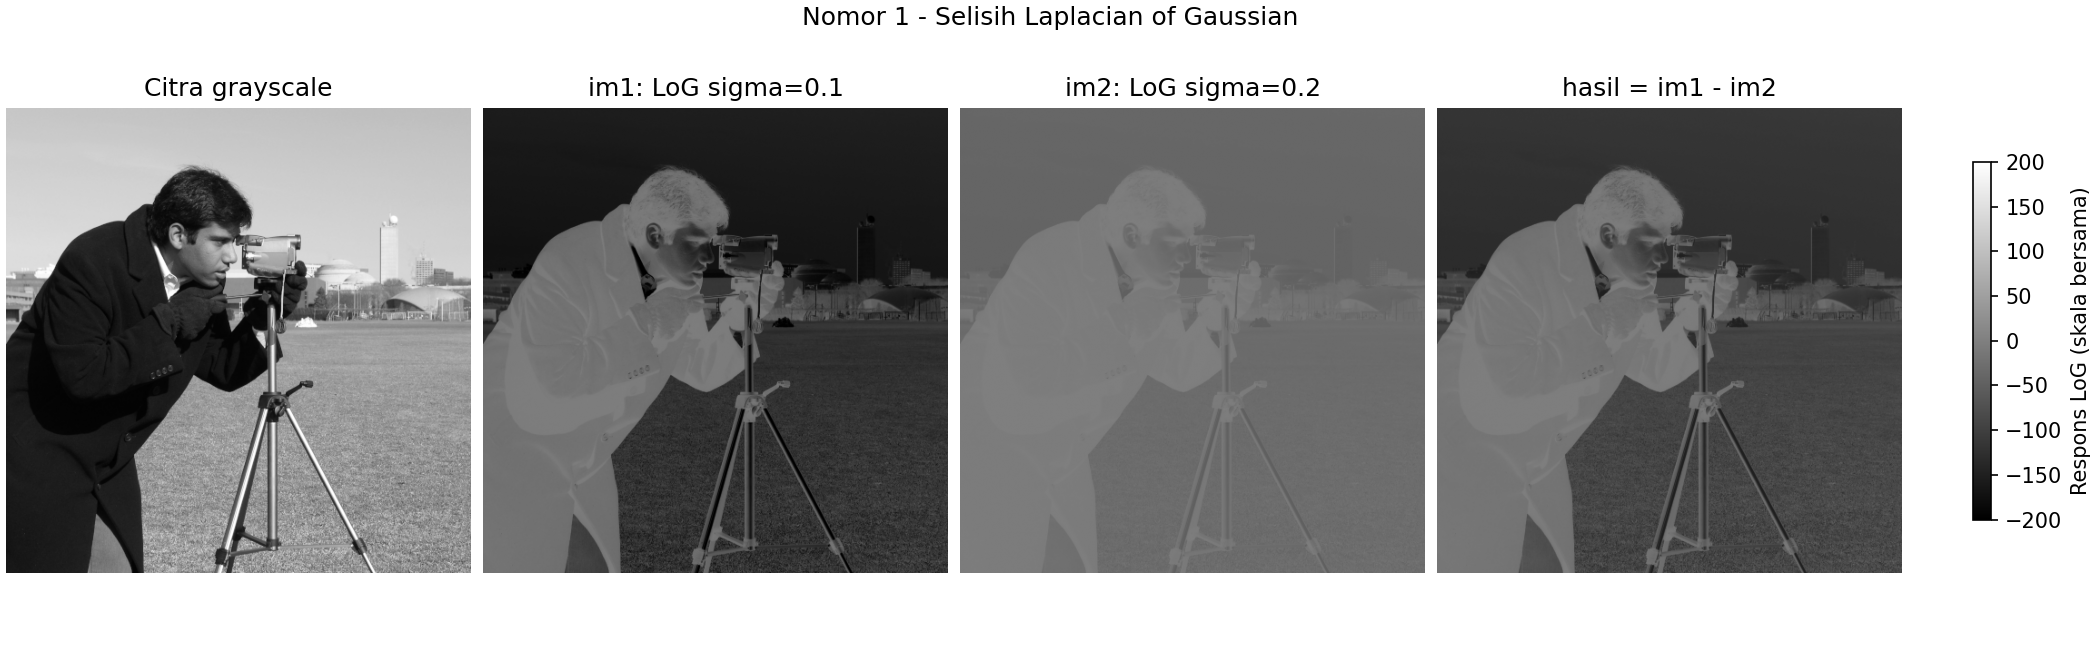
\includegraphics[width=\textwidth]{images/log-foto-nyata.png}
\caption{Dari kiri: foto nyata masukan, respons LoG sigma $0{,}1$,
respons LoG sigma $0{,}2$, dan selisihnya. Ketiga respons menggunakan
skala tampilan bersama.}
\label{fig:log-foto-nyata}
\end{figure}

\begin{table}[H]
\centering
\caption{Rentang respons pada foto nyata, dibulatkan untuk penyajian.}
\begin{tabular}{@{}lrr@{}}
\toprule
\textbf{Array} & \textbf{Minimum} & \textbf{Maksimum}\\
\midrule
\kode{im1} & $-200{,}000000$ & $0{,}000000$\\
\kode{im2} & $-49{,}992070$ & $0{,}000075629$\\
\kode{hasil} & $-150{,}009317$ & $-0{,}000075629$\\
\bottomrule
\end{tabular}
\end{table}

Pemeriksaan array tersimpan menunjukkan bahwa \kode{hasil.npy} sama
persis dengan pengurangan \kode{im1.npy - im2.npy}; ketiganya bertipe
\kode{float64}. Pada foto ini, korelasi selisih terhadap intensitas masukan
sekitar $-0{,}999999999979$. Selisih masih menyerupai negatif foto,
konsisten dengan bias DC akibat sampling kernel pada sigma sangat kecil.
Menggunakan foto nyata tidak menghilangkan keterbatasan tersebut dan
hasil tidak dinyatakan sebagai peta tepi ideal. Data numerik, PNG, dan
metadata tersedia di \kode{soal1/hasil_foto_nyata/}; hasil sintetis
sebelumnya tetap disimpan terpisah.

\clearpage
\section{Penyelesaian Soal Nomor 3: Koin Menurut Ukuran}
\label{sec:soal3}

\subsection{Tujuan, asumsi, dan data percobaan}

Soal nomor 3 meminta penghitungan koin menurut ukurannya dengan bantuan
\kode{skimage.measure.regionprops}~\cite{soal-uts}.
Penyelesaian dilakukan melalui segmentasi, pelabelan komponen, pengukuran
geometri, dan pengelompokan ukuran. Setiap komponen hasil segmentasi
dianggap sebagai satu koin apabila asumsi berikut terpenuhi: koin saling
terpisah, terlihat utuh, memiliki kontras terhadap latar seragam, serta
mayoritas piksel bingkai citra merupakan latar. Seluruh koin dibandingkan
pada skala pengambilan gambar yang sama.

Tidak ada foto koin nyata yang disertakan pada bahan soal yang diterima.
Oleh karena itu, demonstrasi menggunakan citra \textbf{sintetis}
\kode{soal3/data/koin_100.png}, berukuran $1100\times1100$ piksel, yang
dibangkitkan dengan \emph{seed} 9. Citra memuat 100 koin terpisah pada empat
radius, yaitu 13, 18, 23, dan 28 piksel, masing-masing 25 buah. Posisi dan
detail intensitasnya dibuat bervariasi. Informasi pembangkit disimpan pada
\kode{koin_100_ground_truth.json} untuk validasi terpisah; program
penghitung hanya membaca citra dan tidak membaca berkas tersebut.

\subsection{Segmentasi dan pengukuran setiap koin}

Citra masukan dibaca sebagai grayscale atau dikonversi dari RGB ke
grayscale. Untuk RGBA, transparansi dikompositkan pada latar putih terlebih
dahulu. Intensitas grayscale dinormalisasi ke rentang $[0,1]$. Citra yang
seluruh intensitasnya sama ditolak karena tidak menyediakan pemisah antara
objek dan latar.

Ambang $t$ ditentukan menggunakan metode Otsu, yang mencari pemisahan
histogram dengan memaksimumkan variansi antarkelas~\cite{skimage-otsu}.
Mask awal terang didefinisikan sebagai $B(x,y)=[I(x,y)>t]$. Jika sekurangnya
setengah piksel bingkai masuk kelas terang, kelas tersebut dianggap
sebagai latar dan mask objek menjadi komplemen $B$. Jika tidak, $B$
langsung dipakai sebagai mask objek. Dengan aturan ini, koin terang pada
latar gelap maupun koin gelap pada latar terang dapat diproses.

Lubang tertutup pada mask diisi dengan \kode{binary_fill_holes} agar detail
gelap di dalam koin tidak mengurangi luas objek. Komponen diberi label
menggunakan konektivitas 8, kemudian komponen dengan luas kurang dari
50 piksel persegi dibuang. Mask yang tersisa dilabel ulang agar setiap koin
memiliki ID berurutan. Ambang luas tersebut merupakan parameter
\kode{--min-area}, sehingga perlu disesuaikan apabila resolusi citra berubah.

Fungsi \kode{regionprops} menghitung atribut tiap wilayah yang telah
berlabel~\cite{skimage-regions}. Fungsi ini tidak menentukan segmentasi
atau kelas ukuran secara otomatis. Perannya pada program diringkas dalam
Tabel~\ref{tab:regionprops-koin}.

\begin{table}[H]
\centering
\caption{Atribut \kode{regionprops} dan penggunaannya.}
\label{tab:regionprops-koin}
\small
\begin{tabularx}{\textwidth}{@{}p{0.36\textwidth}X@{}}
\toprule
\textbf{Atribut} & \textbf{Penggunaan}\\
\midrule
\kode{label} & ID unik untuk menelusuri objek pada tabel dan anotasi.\\
\kode{area} & Luas objek $A_i$ dalam piksel persegi.\\
\kode{equivalent_diameter_area} & Diameter lingkaran yang luasnya sama
dengan objek; dasar pengelompokan ukuran.\\
\kode{centroid} & Pusat objek untuk menempatkan tulisan ID dan kelompok.\\
\kode{bbox} & Batas kotak objek untuk pemeriksaan lokasi; batas maksimum
mengikuti indeks eksklusif.\\
\bottomrule
\end{tabularx}
\end{table}

Ukuran utama yang digunakan adalah diameter ekuivalen:
\begin{equation}
 d_i=2\sqrt{\frac{A_i}{\pi}}
     =\sqrt{\frac{4A_i}{\pi}}.
 \label{eq:diameter-koin}
\end{equation}
Besaran ini sesuai untuk objek yang mendekati lingkaran dan dinyatakan
dalam piksel. Hasilnya merupakan ukuran geometris pada citra, bukan
diameter dalam milimeter atau nilai nominal mata uang.

\subsection{Aturan pengelompokan dan kode semu}

Diameter diurutkan dari kecil ke besar, dengan ID sebagai pemecah urutan
apabila diameternya sama. Untuk setiap objek, program membentuk calon
kelompok $C$ dengan menambahkan objek tersebut pada kelompok terakhir.
Dengan $m_C=\operatorname{median}\{d_j:j\in C\}$ dan toleransi
$\tau=0{,}08$, penambahan diterima apabila
\begin{equation}
 \lvert d_j-m_C\rvert\leq\tau m_C+10^{-12}
 \quad\text{untuk setiap }j\in C.
 \label{eq:kelompok-koin}
\end{equation}
Jika syarat tidak terpenuhi, objek memulai kelompok baru. Suku sangat
kecil $10^{-12}$ hanya mengantisipasi galat pembulatan numerik. Pemeriksaan
terhadap \emph{seluruh} anggota membatasi efek rantai, yaitu penggabungan
ukuran yang semakin melebar karena perbandingan hanya dilakukan terhadap
objek sebelumnya. Kelompok diberi nama K1, K2, dan seterusnya menurut
ukuran menaik. Jumlah kelompok tidak ditetapkan menjadi empat dan jumlah
objek tidak dipaksa menjadi 100.

\noindent\begin{minipage}{\textwidth}
\begin{lstlisting}[style=pseudocode,caption={Alur penghitungan koin menurut ukuran.}]
INPUT citra I, luas_min = 50, toleransi = 0.08
G = grayscale dan normalisasi I ke [0, 1]
t = ambang_otsu(G)
B = (G > t)
IF fraksi piksel terang pada bingkai >= 0.5:
    M = komplemen B
ELSE:
    M = B
M = isi_lubang(M)
L = label_8_tetangga(M)
Buang komponen dengan luas < luas_min; label ulang
R = regionprops(L)
Urutkan R berdasarkan diameter ekuivalen, kemudian ID
kelompok = daftar kosong
FOR objek dalam R:
    IF kelompok kosong: buat kelompok pertama
    ELSE:
        C = kelompok terakhir ditambah objek
        m = median diameter seluruh anggota C
        IF semua abs(d - m) <= toleransi*m + 1e-12:
            terima objek dalam kelompok terakhir
        ELSE: buat kelompok baru berisi objek
Hitung anggota setiap kelompok
OUTPUT jumlah, pengukuran, mask, label, dan anotasi
\end{lstlisting}
\end{minipage}

Cuplikan berikut memperlihatkan inti pengambilan luas dan diameter dari
\kode{regionprops} dalam implementasi \kode{soal3/main.py}. Program lengkap
juga menyimpan centroid, kotak pembatas, dan nomor kelompok setiap objek.

\noindent\begin{minipage}{\textwidth}
\begin{lstlisting}[style=pythoncode,caption={Inti pengukuran wilayah berlabel.}]
objects = []
for region in measure.regionprops(labels):
    objects.append({
        "id_objek": int(region.label),
        "luas_px2": int(region.area),
        "diameter_ekuivalen_px":
            float(region.equivalent_diameter_area),
    })
\end{lstlisting}
\end{minipage}

\subsection{Hasil dan pembahasan}

Pada citra contoh, ambang Otsu pada intensitas ternormalisasi adalah
$0{,}396484375$. Bingkai dikenali sebagai latar gelap dan tidak ada
komponen yang dibuang oleh penyaringan luas. Hasil pelabelan menghasilkan
100 objek. Pengelompokan dengan toleransi 8\% menghasilkan empat ukuran
dengan jumlah sebagaimana Tabel~\ref{tab:hasil-koin}. Nilai median pada
tabel dibulatkan menjadi dua angka desimal untuk penyajian, sedangkan
\kode{objek_koin.csv} menyimpan pengukuran tanpa pembulatan penyajian.

\begin{table}[H]
\centering
\caption{Hasil penghitungan pada citra koin sintetis dengan \emph{seed} 9.}
\label{tab:hasil-koin}
\small
\begin{tabular}{@{}crrr@{}}
\toprule
\textbf{Kelompok} & \textbf{Diameter pembangkit (px)} &
\textbf{Median terukur (px)} & \textbf{Jumlah}\\
\midrule
K1 & 26 & $25{,}85$ & 25\\
K2 & 36 & $36{,}00$ & 25\\
K3 & 46 & $45{,}95$ & 25\\
K4 & 56 & $55{,}93$ & 25\\
\midrule
\multicolumn{3}{r}{\textbf{Total}} & \textbf{100}\\
\bottomrule
\end{tabular}
\end{table}

\begin{figure}[H]
\centering
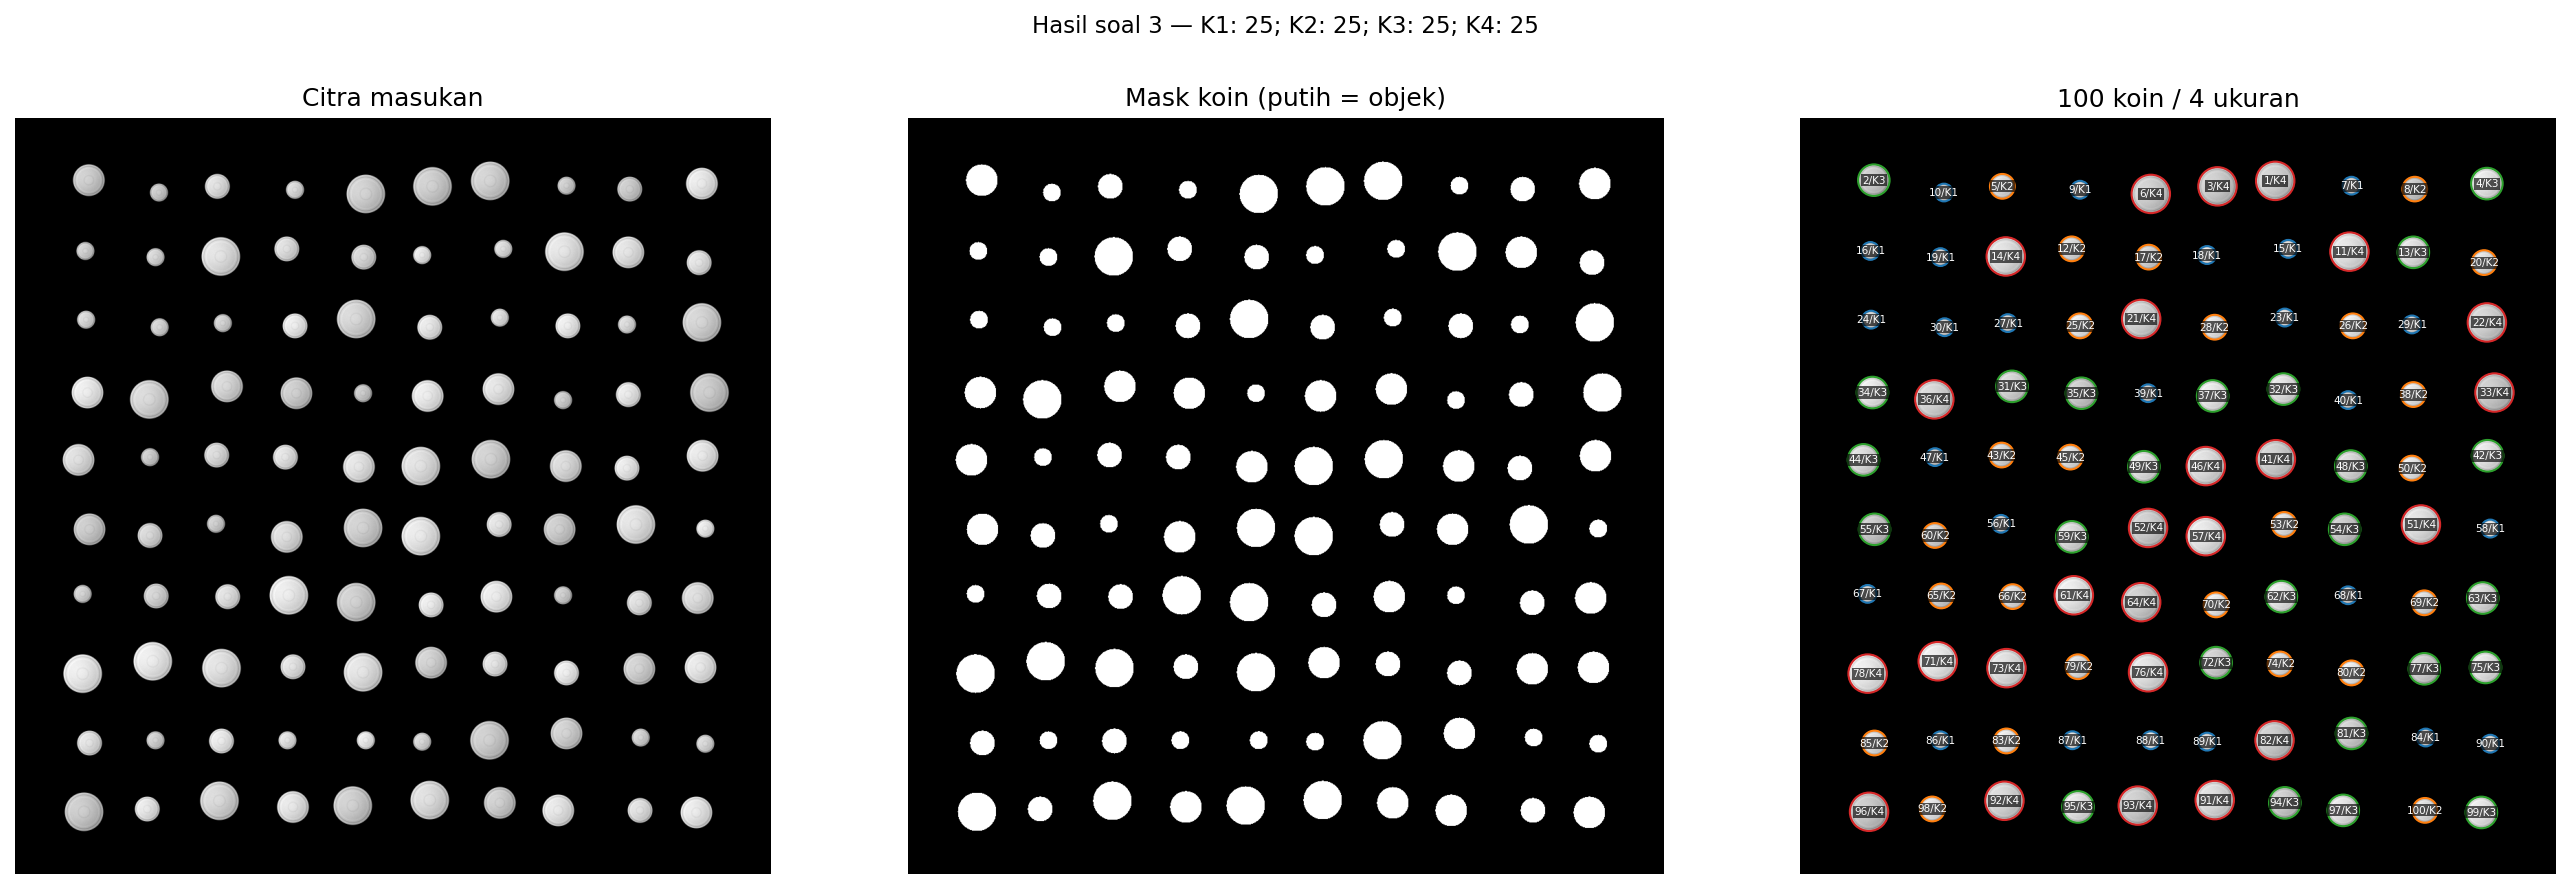
\includegraphics[width=\textwidth]{images/koin-ringkasan.png}
\caption{Citra sintetis, mask segmentasi, dan anotasi hasil.
Tulisan ID/K menunjukkan identitas objek dan kelompok ukurannya.}
\label{fig:koin-ringkasan}
\end{figure}

Jumlah dan distribusi ukuran sesuai dengan metadata pembangkit yang
diperiksa setelah deteksi. Perbedaan kecil antara diameter pembangkit dan
median hasil pengukuran timbul karena diskretisasi piksel, penghalusan
tepi pada citra sintetis, dan keputusan ambang segmentasi. Angka 100 pada
\kode{--expected-count} hanya digunakan untuk mengeluarkan peringatan
apabila jumlah hasil berbeda; parameter ini tidak menambah, menghapus,
atau membagi objek untuk mencapai jumlah tersebut. Statistik kelompok
dan peringatan disimpan pada \kode{ringkasan.json}; mask, label berwarna,
serta anotasi menyediakan bukti visual untuk memeriksa kesalahan.

\subsection{Batasan metode}

Koin bersentuhan dapat bergabung menjadi satu komponen, sedangkan koin
terpotong atau tertutup sebagian menghasilkan diameter yang terlalu
kecil. Pencahayaan tidak seragam, bayangan, dan latar bertekstur dapat
menurunkan mutu ambang global Otsu. Kesalahan pemilihan polaritas juga
mungkin terjadi apabila mayoritas bingkai bukan latar. Perbedaan
perspektif mengubah skala diameter antarlokasi, sementara dua ukuran
fisik yang sangat dekat dapat tergabung akibat toleransi 8\%.
Karena itu, hasil pada data sintetis ini menunjukkan keberhasilan pada
asumsi yang dinyatakan, dan belum membuktikan keandalan pada seluruh
foto koin nyata. Parameter luas minimum dan toleransi ukuran tetap
perlu diperiksa bersama mask dan anotasi ketika memakai citra lain.

\clearpage
\subsection{Pengembangan tambahan: foto dengan pencahayaan tidak merata}
\label{sec:koin-watershed}

Pengembangan ini menguji kondisi di luar asumsi latar seragam pada soal.
Metode utama tetap Otsu. Pilihan \kode{--method watershed} memakai gradien
Sobel sebagai peta batas dan penanda intensitas untuk memisahkan objek
dari latar, mengikuti contoh resmi scikit-image~\cite{skimage-watershed}.
Setelah normalisasi dan penyesuaian polaritas agar objek terang, piksel
dengan intensitas di bawah $0{,}12$ menjadi penanda latar dan piksel di atas
$0{,}6$ menjadi penanda objek. Watershed menentukan kelas piksel sisanya.
Ambang tersebut merupakan parameter awal untuk foto uji, dapat disesuaikan
melalui \kode{--marker-low} dan \kode{--marker-high}, dan tidak berlaku
universal. Pengisian lubang, filter luas, pengukuran \kode{regionprops},
serta pengelompokan ukuran mengikuti tahap berikutnya yang sama.

Foto \kode{skimage.data.coins()} berisi 24 koin, berukuran
$303\times384$ piksel, dan berasal dari koleksi Brooklyn Museum menurut
dokumentasi scikit-image~\cite{skimage-coins}. Foto ini merupakan
\textbf{uji tambahan, bukan pengganti citra utama 100 koin}.

\begin{figure}[H]
\centering
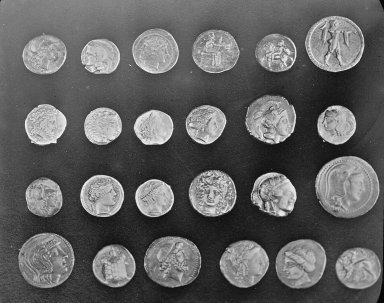
\includegraphics[width=0.31\textwidth]{images/koin-foto-nyata.png}\hfill

\includegraphics[width=0.31\textwidth]{images/koin-mask-otsu.png}\hfill

\includegraphics[width=0.31\textwidth]{images/koin-mask-watershed.png}
\caption{Dari kiri: foto asli, mask Otsu, dan mask watershed. Pada Otsu,
koin kiri atas menyatu dengan latar terang; watershed memisahkannya.}
\end{figure}

Kedua metode menghasilkan 24 region. Namun, jumlah yang sama tidak
menjamin segmentasi benar. Pada Otsu, satu region menggabungkan koin kiri
atas dengan latar, menghasilkan diameter ekuivalen sekitar $109{,}62$ piksel.
Pada watershed, 24 pusat acuan yang ditandai secara visual masing-masing
berada pada region berbeda, dengan selisih centroid kurang dari 3 piksel;
seluruh kotak pembatas juga terpisah dari bingkai. Ini memeriksa lokasi
dan identitas objek, bukan ketepatan setiap piksel mask atau diameter fisik.
Lima kelompok diameter piksel berjumlah 10, 8, 2, 3, dan 1; kelompok
tersebut belum divalidasi sebagai kategori ukuran fisik atau nominal uang.

\begin{lstlisting}[style=terminal]
.\.venv\Scripts\python.exe soal3/main.py --input soal3/data/koin_nyata_scikit.png --method watershed --expected-count 24 --output-dir soal3/hasil_foto_nyata_watershed
\end{lstlisting}

Pemeriksaan tambahan mencakup foto ini serta citra dengan gradien latar
dan inversi intensitas. Metode tetap memerlukan penanda yang sesuai dan
koin terpisah; belum menjamin keberhasilan pada semua pencahayaan atau
latar bertekstur. Pada metode bawaan, mask dan CSV pengukuran 100 koin
sintetis tetap identik dengan hasil sebelum pengembangan.

\clearpage
\section{Reproduksi dan Pengujian}
\label{sec:reproduksi}

\subsection{Lingkungan eksekusi}
Program menggunakan Python 3.10 atau lebih baru. Eksekusi yang diperiksa
menggunakan Python 3.10, NumPy 2.2.6, SciPy 1.15.3, scikit-image 0.25.2,
Matplotlib 3.10.9, dan Pillow 12.3.0. Semua dependensi program dicantumkan
di \path{requirements.txt}; dependensi pengujian tambahan tercantum pada
\path{requirements-dev.txt}.

Satu cara eksekusi digunakan secara konsisten, yaitu melalui Python di
\kode{.venv}. Dari folder utama repositori pada Windows PowerShell,
persiapan berikut cukup dilakukan sekali:
\begin{lstlisting}[style=terminal]
python -m venv .venv
.\.venv\Scripts\python.exe -m pip install -r requirements.txt
\end{lstlisting}
Setelah dependensi terpasang, jalankan ketiga program:
\begin{lstlisting}[style=terminal]
.\.venv\Scripts\python.exe soal1/main.py
Push-Location soal2
..\.venv\Scripts\python.exe main.py
Pop-Location
.\.venv\Scripts\python.exe soal3/main.py
\end{lstlisting}
Pemanggilan langsung interpreter tersebut tidak memerlukan aktivasi
lingkungan. Folder \kode{.venv} dibuat pada masing-masing komputer dan
diabaikan oleh Git.

Nomor 2 dijalankan dari folder \kode{soal2/} karena lokasi masukan
dan keluaran mengikuti folder kerja. Tutup jendela visualisasi agar terminal
dapat melanjutkan. Kode pekerjaan Dustin dipertahankan.

\subsection{Berkas keluaran}
Hasil nomor 1 tersimpan di \path{soal1/hasil/}. Berkas \kode{im1.npy},
\kode{im2.npy}, dan \kode{hasil.npy} menyimpan data numerik bertanda.
Berkas PNG merupakan visualisasi, sedangkan \kode{metadata.json}
menyimpan parameter dan statistik respons.

Hasil nomor 2 tersimpan di \path{soal2/hasil_karakter/}: 18 gambar
karakter serta \kode{_visualisasi_bbox.png}. Pemeriksaan eksekusi dan hasil
nomor 2 dijelaskan pada Bagian~\ref{sec:soal2}; tidak termasuk dalam
tes otomatis nomor 1 dan 3.

Hasil nomor 3 tersimpan di \path{soal3/hasil/}. Berkas \kode{mask_koin.png}
menunjukkan segmentasi; \kode{label_koin.png} membedakan objek;
\kode{anotasi_koin.png} menunjukkan ID dan kelompok. Pengukuran tiap objek
tersimpan di \kode{objek_koin.csv}, sedangkan jumlah serta statistik setiap
kelompok tersimpan di \kode{ringkasan.json}.

\subsection{Pemeriksaan otomatis}
Dua belas pengujian mencakup tiga pemeriksaan LoG, lima pemeriksaan koin
inti, dan empat kasus pengembangan watershed. Pengujian dilakukan dengan:
\begin{lstlisting}[style=terminal]
.\.venv\Scripts\python.exe -m pip install -r requirements-dev.txt
.\.venv\Scripts\python.exe -m pytest -q
\end{lstlisting}

\begin{table}[H]
\centering
\caption{Cakupan dan hasil delapan pengujian inti.}
\label{tab:pengujian}
\small
\begin{tabularx}{\textwidth}{@{}p{0.7cm}Xp{1.2cm}@{}}
\toprule
\textbf{No.} & \textbf{Pemeriksaan} & \textbf{Hasil}\\
\midrule
1 & LoG pada citra konstan $0{,}4$ dengan $\sigma=0{,}1$ menghasilkan $-80$. & Lulus\\
2 & Dua respons dengan sigma sama mempunyai selisih nol persis. & Lulus\\
3 & Impuls pada sigma 1 dan 2 menghasilkan respons bertanda; penyimpanan
\kode{.npy} mempertahankan pengurangan. & Lulus\\
4 & Seluruh 100 objek dipasangkan ke pusat acuan; diameter dan kelompok
ukurannya sesuai toleransi pemeriksaan. & Lulus\\
5 & Inversi intensitas, sehingga latar menjadi terang, mempertahankan
deteksi dan kelompok seluruh koin. & Lulus\\
6 & Resolusi setengah mempertahankan jumlah dan kelas; diameter mengikuti
perubahan skala. & Lulus\\
7 & Lubang diisi dan derau kecil dibuang pada contoh sembilan koin; hasil
dua kelompok berjumlah tujuh dan dua. & Lulus\\
8 & Citra seragam dan berkas citra kosong ditolak dengan pesan kesalahan. & Lulus\\
\bottomrule
\end{tabularx}
\end{table}

Empat kasus tambahan mencakup kesesuaian mask pada gradien latar dengan
dua polaritas, pemetaan satu per satu terhadap 24 pusat koin foto nyata,
dan penolakan penanda watershed tidak valid atau kosong. Pada citra
gradien sintetis, rasio irisan terhadap gabungan mask acuan lebih dari
$0{,}94$. Hasil seluruh pengujian adalah \texttt{12 passed}.
Pengujian pada sigma 1 dan 2
merupakan pemeriksaan tambahan terhadap penyimpanan nilai bertanda;
hasil utama nomor 1 tetap memakai sigma $0{,}1$ dan $0{,}2$.
Contoh sembilan koin menunjukkan bahwa jumlah hasil tidak dipaksa menjadi
100. Keberhasilan pada data sintetis tidak menyatakan akurasi universal
pada foto nyata dengan pencahayaan, perspektif, atau latar yang berbeda.

\section{Kesimpulan}
Program nomor 1 membaca citra, menghitung dua respons LoG pada
$\sigma=0{,}1$ dan $\sigma=0{,}2$ piksel, lalu menyimpan selisih
\texttt{im1 - im2} sebagai data float64 bertanda. Visualisasi dibuat setelah
pengurangan, sehingga penyesuaian tampilan tidak mengubah hasil numerik.
Sigma yang sangat kecil menyebabkan bias respons pada grid diskret;
hal tersebut perlu dibedakan dari perilaku ideal LoG kontinu.

Program nomor 2 memakai komponen terhubung dan \kode{regionprops}
untuk memisahkan 18 karakter pada citra contoh menjadi berkas individual.
Mask tiap region mempertahankan orientasi karakter dan menghindari
penyalinan karakter tetangga di dalam kotak pembatas.

Program nomor 3 memisahkan koin melalui ambang Otsu dan komponen
terhubung, mengukur luas serta diameter ekuivalen menggunakan
\kode{regionprops}, kemudian menghitung jumlah tiap kelompok ukuran.
Pada contoh sintetis, diperoleh 100 koin dalam empat kelompok, masing-masing
25 buah. Delapan pengujian lulus. Penerapan bergantung pada asumsi koin
terpisah, terlihat utuh, dan kontras terhadap latar seragam.

\clearpage
\begin{thebibliography}{9}
\raggedright
\small
\setstretch{1}
\setlength{\itemsep}{3pt}
\setlength{\parskip}{0pt}
\addcontentsline{toc}{section}{Daftar Pustaka}
\bibitem{soal-uts}
Peter Rhatodirdjo Angka,
\textit{UTS INF301 Pengolahan Citra Digital, Semester Gasal 2026/2027}.
Program Studi Informatika, Fakultas Teknik, Universitas Katolik Widya
Mandala Surabaya, 8 Oktober 2026. Dokumen soal yang diberikan.

\bibitem{scipy-log}
SciPy Developers,
\textit{scipy.ndimage.gaussian\_laplace}.
Dokumentasi resmi SciPy.
\href{https://docs.scipy.org/doc/scipy/reference/generated/scipy.ndimage.gaussian_laplace.html}{Tersedia pada laman resmi SciPy}.

\bibitem{skimage-regions}
scikit-image Developers,
\textit{skimage.measure.regionprops}.
Dokumentasi resmi scikit-image.
\href{https://scikit-image.org/docs/stable/api/skimage.measure.html#skimage.measure.regionprops}{Tersedia pada laman resmi scikit-image}.

\bibitem{skimage-otsu}
scikit-image Developers,
\textit{skimage.filters.threshold\_otsu}.
Dokumentasi resmi scikit-image.
\href{https://scikit-image.org/docs/stable/api/skimage.filters.html#skimage.filters.threshold_otsu}{Tersedia pada laman resmi scikit-image}.
\end{thebibliography}


\end{document}
